\subsection{Example: Bayesian Regularized Neural Network}

This example returns to the Tohoku Earthquake problem, offering another potential solution.  It uses the \texttt{brnn} package to fit a neural network with Bayesian regularization by means as described above and in further detail by (Mackay, 1992).  Data was not divided into a test set to assess predictive accuracy, although it can be in the same manner as was done earlier.  Rather than assessing predictive accuracy here, an alternate approach will be introduced later.  This example serves merely as direct exposure to the regularization techniques described.

The model is a 6-layer Bayesian Regularized Neural Network (BRNN) to make a prediction for a magnitude 9.1 earthquake in the Tohoku area.  Its syntax is relatively simple, with many defaults that can be modified for special cases.  The default optimization is the Gauss-Newton optimization algorithm (Forsee and Hagan, 1997).

\begin{Shaded}
\begin{Highlighting}[]
\NormalTok{x }\OtherTok{\textless{}{-}}\NormalTok{ earthquakes\_log}\SpecialCharTok{$}\NormalTok{mag}
\NormalTok{y }\OtherTok{\textless{}{-}}\NormalTok{ earthquakes\_log}\SpecialCharTok{$}\NormalTok{freqc}

\NormalTok{brnn }\OtherTok{\textless{}{-}} \FunctionTok{brnn}\NormalTok{(y}\SpecialCharTok{\textasciitilde{}}\NormalTok{x,}\AttributeTok{neurons=}\DecValTok{6}\NormalTok{)   }
\end{Highlighting}
\end{Shaded}

\begin{verbatim}
## Number of parameters (weights and biases) to estimate: 18 
## Nguyen-Widrow method
## Scaling factor= 4.2 
## gamma= 6.6171     alpha= 0.1129   beta= 869.274
\end{verbatim}

\begin{Shaded}
\begin{Highlighting}[]

\FunctionTok{summary}\NormalTok{(brnn)            }\CommentTok{\# summary of model}
\end{Highlighting}
\end{Shaded}

\begin{verbatim}
## A Bayesian regularized neural network 
## 1 - 6 - 1 with 18 weights, biases and connection strengths
## Inputs and output were  normalized
## Training finished because  Changes in F= beta*SCE + alpha*Ew in last 3 iterations less than 0.001
\end{verbatim}
\begin{comment}
The above output describes the model in text.  Notationally, the model is given (as imputed into the general formula from the \texttt{brnn} package documentation) by:
$$
\hat{y_i} = \sum_{k=1}^6 w_k g_k (b_k + \sum_{j=1}^{31} x_{ij} \beta_j^{[k]} ) + e_i
$$

\begin{gather*}
e_i \sim N(0,\sigma^2) \\
w_k \text{ is the weight of the } k^{th} \text{ neuron} \\
b_k \text{ is the bias of the } k^{th} \text{ neuron} \\
\beta_j^{[k]} \text{ is the weight of the } j^{th} \text{ input to the net} \\
g_k \text{ is the activation function } g_k(x) = \frac{e^{2x}-1}{e^{2x}+1}
\end{gather*}
\end{comment}

\begin{Shaded}
\begin{Highlighting}[]
\CommentTok{\# return interval of years based on 9.1 prediction}
\NormalTok{b }\OtherTok{\textless{}{-}} \FunctionTok{predict}\NormalTok{(brnn, }\AttributeTok{newdata =} \FunctionTok{data.frame}\NormalTok{(}\AttributeTok{x =} \FloatTok{9.1}\NormalTok{)) }
\DecValTok{1}\SpecialCharTok{/}\NormalTok{(}\DecValTok{10}\SpecialCharTok{\^{}}\NormalTok{b) }
\end{Highlighting}
\end{Shaded}

\begin{verbatim}
## [1] 106.9823
\end{verbatim}

Using this neural network model, the expected frequency of a magnitude
9.1 earthquake would be one every 106.98 years.  This may be an alarming catch to the Fukushima engineering officials!  And indeed they may aim to design a stronger reactor. A plot of the data is shown below:

\begin{comment}

\hypertarget{plots-for-brnn}{%
\subsubsection{plots for brnn}\label{plots-for-brnn}}

\begin{Shaded}
\begin{Highlighting}[]
\CommentTok{\#{-}{-}{-}actual test data{-}{-}{-}}
\NormalTok{actual\_log\_brnn }\OtherTok{\textless{}{-}}\NormalTok{ earthquakes\_log }\SpecialCharTok{\%\textgreater{}\%} 
  \FunctionTok{mutate}\NormalTok{(}\AttributeTok{type =} \StringTok{"actual"}\NormalTok{)}
 \CommentTok{\# add\_row(mag = addt, freqc = NA, type = "actual")}

\CommentTok{\#{-}{-}{-}predicted data{-}{-}{-}}
\NormalTok{mdp }\OtherTok{\textless{}{-}} \FunctionTok{seq}\NormalTok{(}\DecValTok{8}\NormalTok{,}\FloatTok{9.1}\NormalTok{, }\AttributeTok{by =}\NormalTok{ .}\DecValTok{1}\NormalTok{) }\CommentTok{\#additional magnitude data points to add to prediction data}

\NormalTok{bnn\_preds }\OtherTok{\textless{}{-}}\NormalTok{ earthquakes\_log}\SpecialCharTok{$}\NormalTok{mag }\SpecialCharTok{\%\textgreater{}\%} \FunctionTok{append}\NormalTok{(mdp) }\CommentTok{\#append additional magnitudes to make predictions}

\NormalTok{predicted\_log\_brnn }\OtherTok{\textless{}{-}} \FunctionTok{data.frame}\NormalTok{(}\AttributeTok{mag =}\NormalTok{ bnn\_preds,}
                             \AttributeTok{freqc =} \FunctionTok{predict}\NormalTok{(brnn, }\AttributeTok{newdata =} \FunctionTok{data.frame}\NormalTok{(}\AttributeTok{x =}\NormalTok{ bnn\_preds)),}
                             \AttributeTok{type =} \StringTok{"predicted"}\NormalTok{)}


\CommentTok{\#{-}{-}{-}combine test and predictions for plot{-}{-}{-}}
\NormalTok{brnn\_plot }\OtherTok{\textless{}{-}} \FunctionTok{rbind}\NormalTok{(predicted\_log\_brnn,actual\_log\_brnn[,}\FunctionTok{c}\NormalTok{(}\DecValTok{1}\NormalTok{,}\DecValTok{3}\NormalTok{,}\DecValTok{4}\NormalTok{)])}

\CommentTok{\#{-}{-}{-}generate plot{-}{-}{-}}
\FunctionTok{ggplot}\NormalTok{(brnn\_plot, }\FunctionTok{aes}\NormalTok{(}\AttributeTok{x =}\NormalTok{ mag, }\AttributeTok{y =}\NormalTok{ freqc, }\AttributeTok{group =}\NormalTok{ type, }\AttributeTok{color =}\NormalTok{ type)) }\SpecialCharTok{+}
  \FunctionTok{geom\_line}\NormalTok{() }\SpecialCharTok{+}
  \FunctionTok{geom\_point}\NormalTok{(}\AttributeTok{size =} \DecValTok{2}\NormalTok{, }\AttributeTok{shape =} \DecValTok{17}\NormalTok{ , }\AttributeTok{alpha =}\NormalTok{ .}\DecValTok{5}\NormalTok{) }\SpecialCharTok{+}
  \FunctionTok{theme\_minimal}\NormalTok{() }\SpecialCharTok{+}
  \FunctionTok{labs}\NormalTok{(}\AttributeTok{x =} \StringTok{"Magnitude"}\NormalTok{,}
       \AttributeTok{y =} \StringTok{"Annual Frequency of At Least this Magnitude"}\NormalTok{,}
       \AttributeTok{title =} \StringTok{"Annual Earthquake Frequency near Tohoku, Japan {-} Logarithmic Scale"}\NormalTok{,}
       \AttributeTok{subtitle =} \StringTok{"Three{-}Layer Neural Network with Bayesian Regularization"}\NormalTok{)}
\end{Highlighting}
\end{Shaded}

\end{comment}

\begin{figure}[H]
    \center
    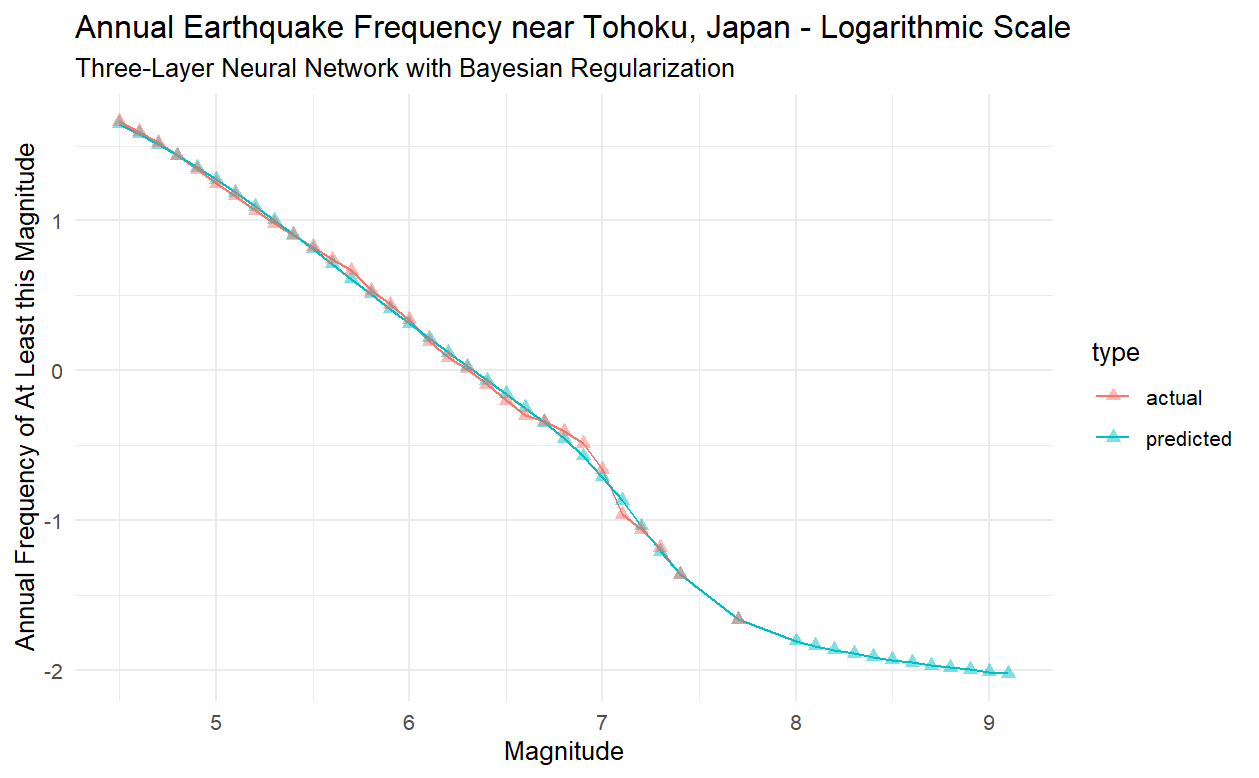
\includegraphics[width=0.8\linewidth]{Figures/tohoku_logscale_brnn.png}
   % \vspace{-10pt}
    \caption{\footnotesize{Actual data points plotted with BRNN-predicted values for all data points, with appended predicted magnitudes for sequential series of magnitude 8.0 - 9.1 by 0.1}}
    \label{tohoku_brnn}
\end{figure}

Suppose the Fukushima engineering officials are not as astonished as anticipated; instead they simply ask, ``How certain are we about this prediction?''  This model by itself is not able to answer that question. 
%It lacks the additional scaffolding described in earlier sections.  In the next and final chapter, the remaining techniques for practical neural network modeling will incorporate the Bayesian techniques learned in this chapter with predictive accuracy measures.  The final example will further embellish the prediction at hand and tell the story to the engineers.
However, in implementing the full stochastic effect of a Bayesian Neural Network, multiple iterations of the same model can be trained and plotted in the same manner as before.  Figure \ref{tohoku_brnn_uncert} displays 100 individually trained networks of the same architecture plotted to show relative uncertainty in its prediction curvature, as well as the scatter of predictions for lapsed time between earthquakes of magnitude 9.1 for the same 100 models.

\begin{figure}[H]
%    \center
    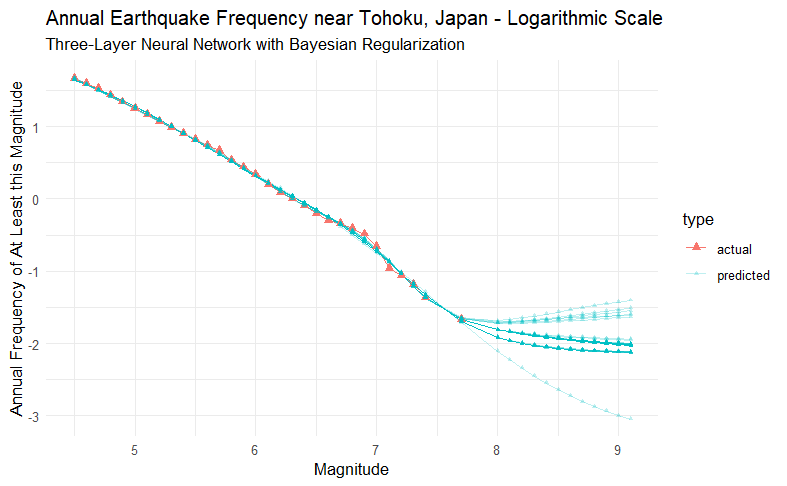
\includegraphics[width=0.5\linewidth]{Figures/tohoku_logscale_brnn_uncert.png}
    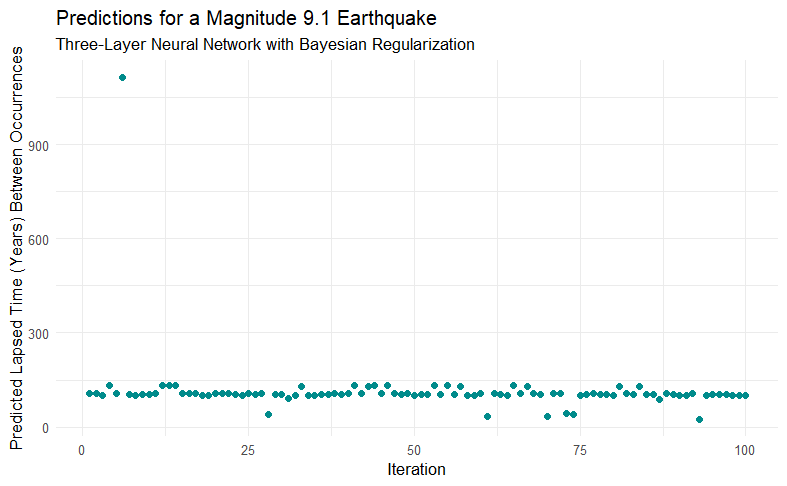
\includegraphics[width=0.5\linewidth]{Figures/tohoku_9.1preds_scatter.png}
   % \vspace{-10pt}
    \caption{\footnotesize{[\textit{left}] Actual data points plotted with multiple BRNN-predicted values, with uncertainty captured by the positions of individual model curves. [\textit{right}] Scatter of predictions of a magnitude 9.1 earthquake, rescaled to represent predicted frequencies of occurrence.}}
    \label{tohoku_brnn_uncert}
\end{figure}

With further use of data visualization tools, the \textit{underlying distribution of predictions} can be observed.  Figure \ref{tohoku_ppd_100} shows the cumulative distribution of all 100 iterations of the predicted frequency of a magnitude 9.1 earthquake, which includes one very incongruous point.  For no more purpose other than to better visualize the area with the most density, this point was temporarily removed.

\begin{figure}[H]
%    \center
    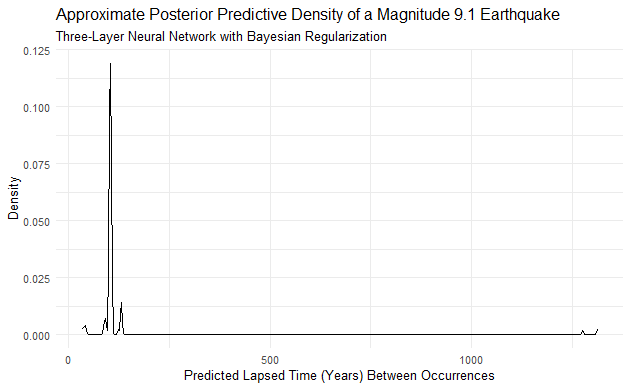
\includegraphics[width=0.5\linewidth]{Figures/tohoku_ppd_full.png}
    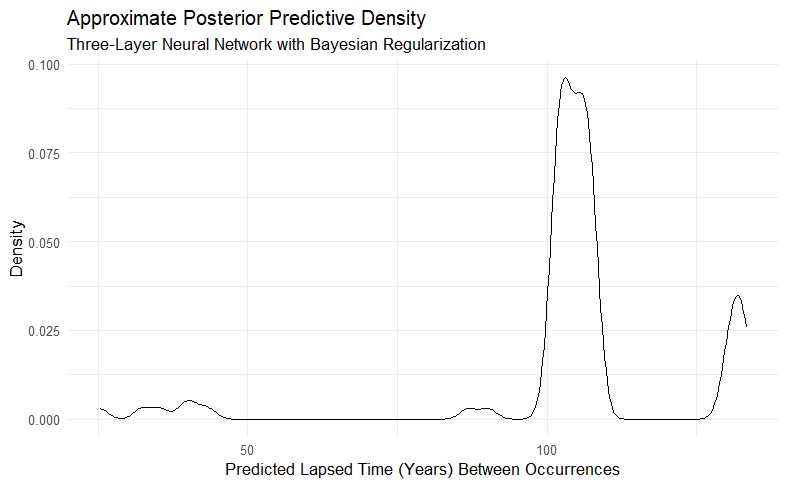
\includegraphics[width=0.5\linewidth]{Figures/tohoku_ppd_99obs.png}
   % \vspace{-10pt}
    \caption{\footnotesize{[\textit{left}] Full cumulative distribution of predicted magnitude 9.1 frequency values for all 100 iterations. [\textit{right}] Refined view showing 99\% of the density.}}
    \label{tohoku_ppd_100}
\end{figure}

Next, 1000 networks of identical architecture are trained and a clearer distribution displayed.  As the number of simulated networks increases, the approximation for the \textit{true posterior predictive distribution of the expected frequency of a magnitude 9.1 earthquake}
$P(y|x=9.1,D)$
more closely represents the target distribution.


\begin{figure}[H]
    \center
    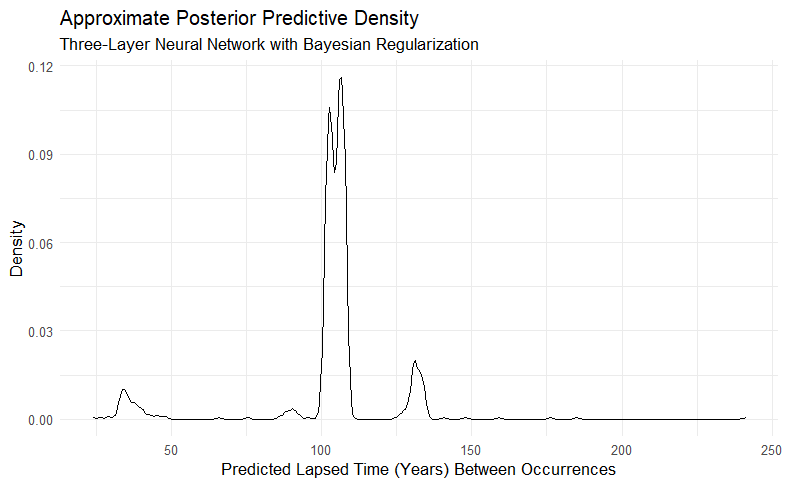
\includegraphics[width=0.8\linewidth]{Figures/tohoku_ppd_995.png}
   % \vspace{-10pt}
   \caption{\footnotesize{Refined view of 1000 model iterations showing 99.5\% of the density for predicted magnitude 9.1 frequency. }}
    \label{tohoku_ppd_1000}
\end{figure}